\section{WebCMS (https://webcms3.cse.unsw.edu.au/)}

WebCMS is a LMS designed and used internally for UNSW CSE courses. WebCMS is a browser based LMS that allows unauthenticated users to only see course announcement page and other pages require an authenticated user with correct enrolment access to the course.

\subsection{Enrolments}
WebCMS has a robust enrolment system that is managed by lecturers and course admins. Course Staff creates a course for a specific term and enrols students from enrolment list. Students can be enrolled into multiple courses for each term.

\begin{itemize}
	\item WebCMS has multiple roles that can be assigned to individuals for specific courses (Lecturers, Students, Tutors, Course Admin). Each page in the course can be customised to be accessible by users with specific roles.
	\item Users enrolled into multiple courses will be able to navigate through the courses via the nav bar at top of page. Users can have different roles for each course. (Student in course A and Tutor in course B)
\end{itemize}
\newpage

\begin{figure}[h!]
    \centering
    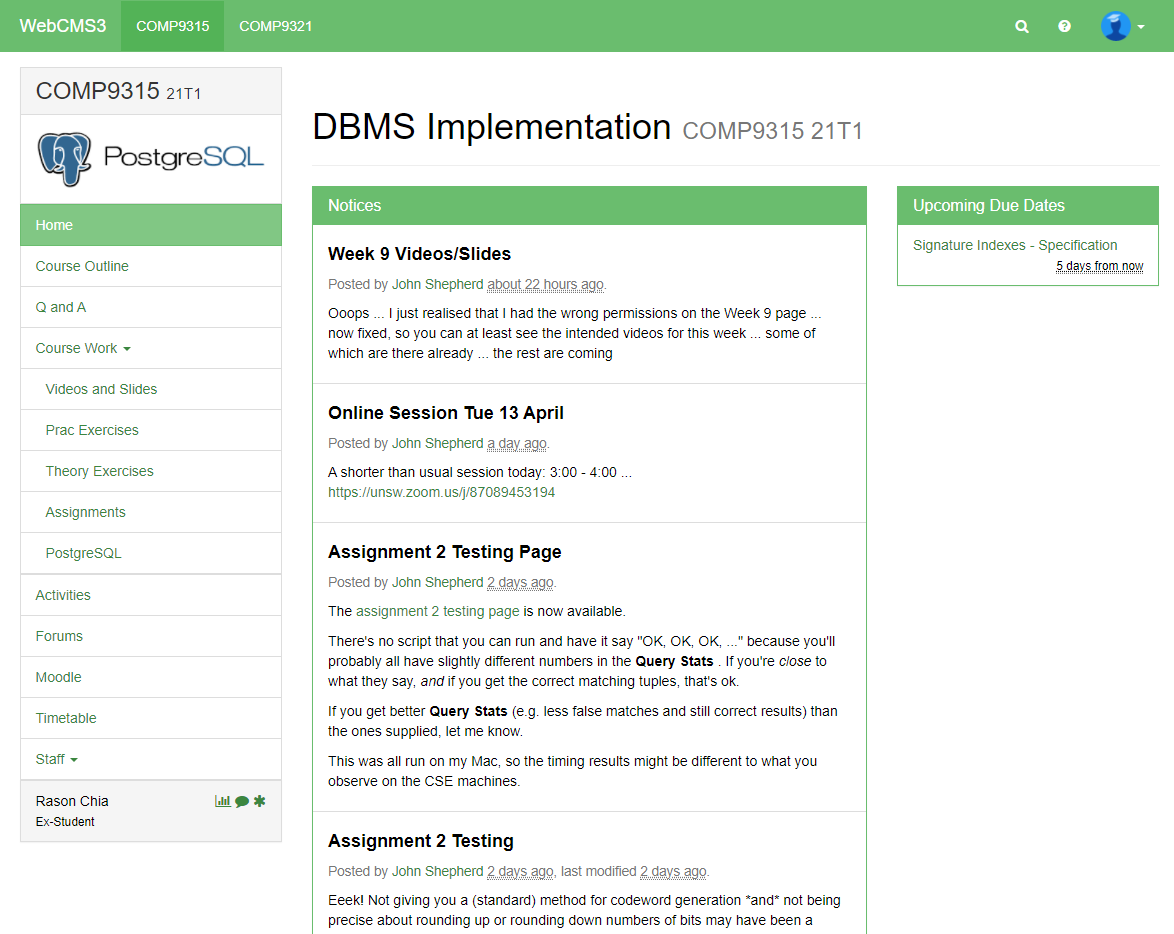
\includegraphics[scale=0.6]{webcms-coursepage}
    \caption{WebCMS's Student Course Page}
\end{figure}

\subsection{Course Page Feed}
Each Course has a homepage that users will land on when navigating to the course. This main page consists of 3 main components, a static navbar to navigate course content, Course Notices / Announcements and due dates for deliverables.

\begin{itemize}
	\item Course Notices / Announcements can be posted by lecturers or staff member. These posts will automatically generate an email notification to all enrolled users of the course. Posts are visible to all users and provide course wide information like release of assignments and exam information.
	\item Due dates of deliverables are retrieved from quizes and assignments that have a due date set. The panel will show the number of days remaining as well as a link to the specific deliverable.
	\item The static sidebar provides an indexed view of course content. Content links can be grouped under a heading. This allows users to quickly navigate through to the content they are looking for. This sidebar also display the authenticated user's name, role in the course, shortcut links to user's gradebook, wiki and blog.
	\item Course Admins can set course theme color which is propagated through all the above elements as well as throughout all pages for the specific course. Each course can have a different theme color and this helps users differentiate which course they are looking at.
\end{itemize}

\subsection{Email Notifications}
WebCMS has a email notification feature which can be triggered automatically on various conditions. By default, any course wide notices always striggers email notifications.
\begin{itemize}
\item Users have the eability to subscribe to their posts (comments, replies, forum posts) which will automatically triggger notifications if there has been a new update to their posts. This can be toggled in the settings menu.
\end{itemize}

\subsection{Quiz and Assignment System}
WebCMS allows multiple quizes and assignments to be created for each course. These deliverables have a due date and can be fully customised, automarked and results displayed directly into the user's gradebook.

\begin{itemize}
	\item Quizes can comprise of only multiple choice answers or have a mix with short \& long response answers. Correct answers can be set for each quiz, once quiz is due, users are not allowed to make anymore submissions and quizes can be automatically marked by WebCMS.
	\item Assignments can be created with multiple tabs (Specification, Make Submission, Check Submission, Collect Submission). Specification can be formatted or displayed through embedded pdf. Make, Check and Collect Submission functionalities interacts with CSE give command line tools for specific assignment.
\end{itemize}

\subsection{Display Content}
WebCMS has a robust page formatting toolset which allows the user to format content with headers, create lists and embed content (videos, images).

\begin{itemize}
	\item Course Setting can restrict that only lecturers or staff members can create or edit the page.
	\item Pages created can be pinned into the static navbar on the platform for easy access
	\item Pages can be access by direct link to its content resource number that is unique to each page. e.g. \url{https://webcms3.cse.unsw.edu.au/COMP9321/21T1/resources/59281}
	\item Pages can be embedded with pdf files which provides a basic pdf viewer component so users can view pdfs while remaining on the platform
\end{itemize}

\subsection{Gradebook and Profile}
WebCMS gradebook stores marks from deliverables like quizes, labs, assignments. User Profiles also has a blog and wiki feature where users can document notes as well as store a blurb about themselves which is visible to other users.

\begin{itemize}
	\item Quizes which are set to automark can record their scores automatically into the gradebook.
	\item Marks for Quizes, Labs and Assignments can be manually inputted into the gradebook for each user. This feature can be restricted to be used by staff members only.
	\item Gradebook allows for total of specfic marks to be displayed on the gradebook. This is done to provide a summary view of a student's score over all the deliverables.
\end{itemize}

\subsection{Admin Functionalities}
WebCMS administrative functionalities can be restricted to certain user groups like staff members. Admin Functions allow staff members to create and manage course content \& structures.

\begin{itemize}
	\item Course Creation Tools: Creating Brand New Courses and Stetup, Cloning previous courses, Link Course to myunsw enrolment course student lists
	\item Course Management Tools: Setup deliverables for the course (Quizes, Assignments, Labs), Setup Course Content (Lecture Slides, Labs, Assignment Pages, Quiz Questions), 
	\item Student Interaction Tools: Setup pages to have commenting functionality, Setup forums, Setup Notification Settings
\end{itemize}

\subsection{Conclusion}
WebCMS is a comprehensive and robust Learning Management System, however it does fall short of some other LMS in the market. WebCMS is not an open source platform that can easily recieve external data or export its own data, it is built as a platform to store / share content but it does not engage students directly with any self serve content like gamification features or self serve modules.